\section{Fatto in tesi}
\subsection{Filogenesi iqtree nucleotidi}
Dataset: 186 geni BUSCO single copy in almeno 43/48 specie (90\%).

\begin{figure}[ht]
    \centering
    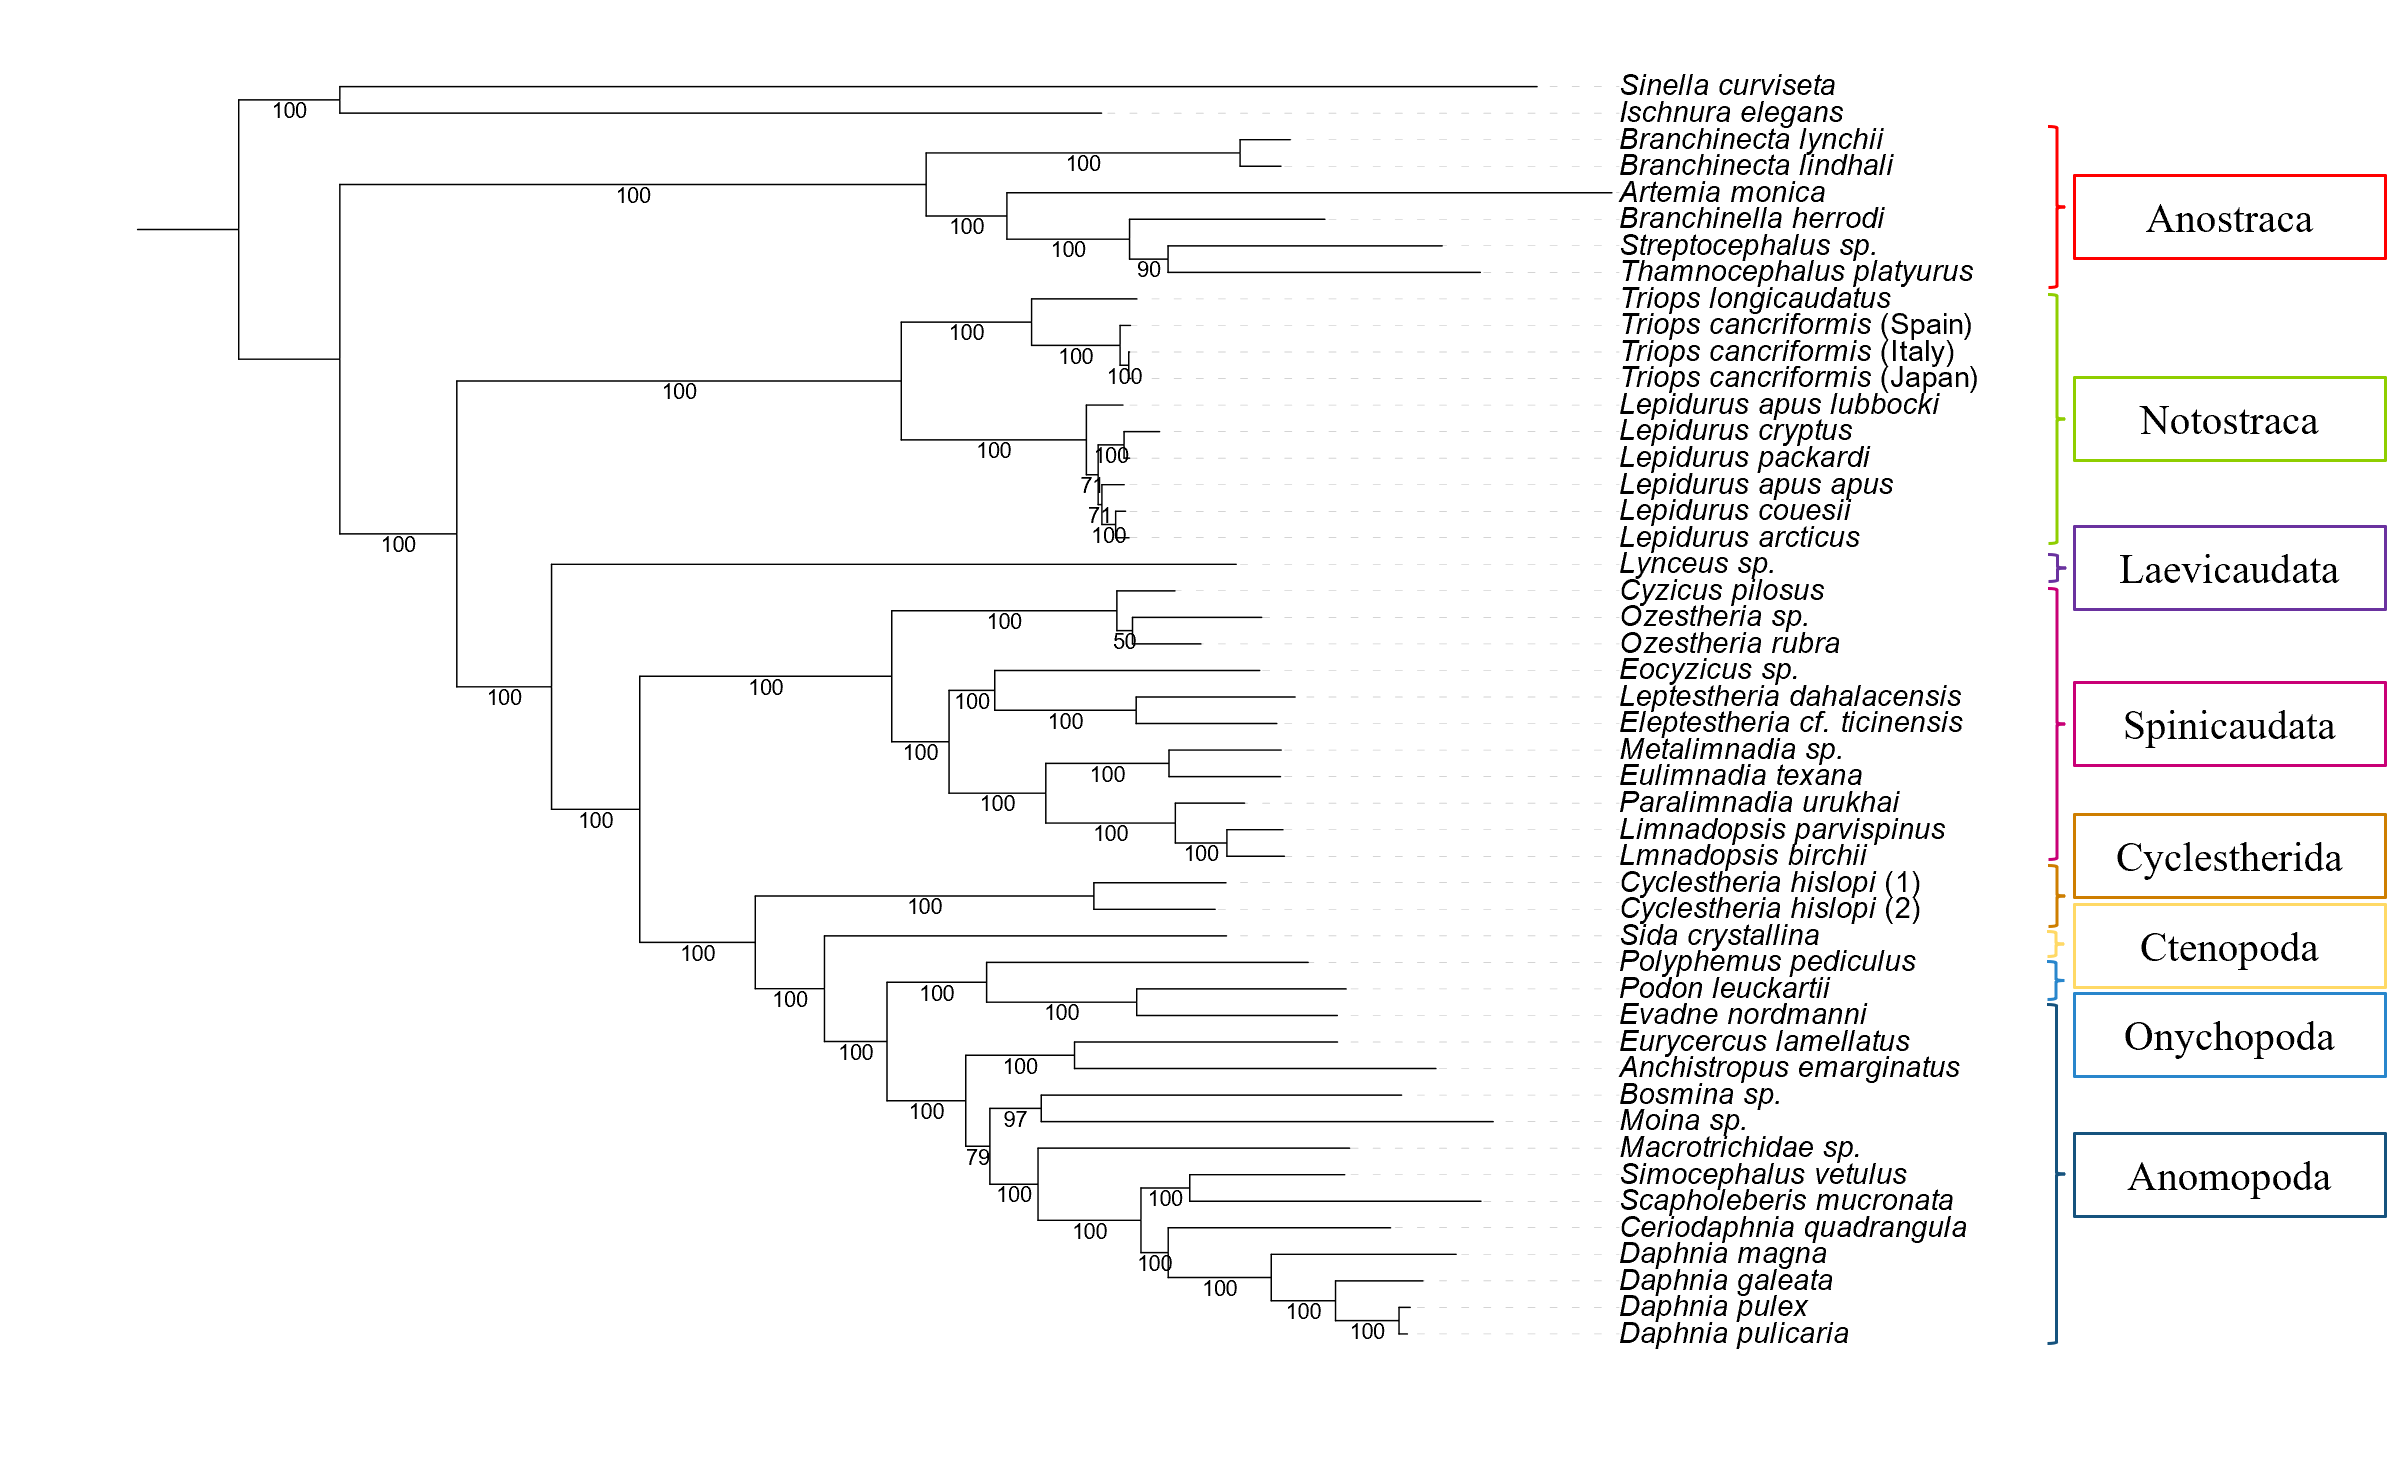
\includegraphics[width=1\textwidth]{Figures/busco_tree_fna.png}
    \caption[BUSCO phylogeny]{Maximum likelihood phylogenetic tree built on the nucleotide alignment of the 186 BUSCO genes present in at least 90\% of the species (43/48) using IQ-TREE. Numbers at branches represent ultrafast bootstrap proportion.
}
    \label{fig:busco_phylo}
\end{figure}

\newpage
\subsection{Dating sui nucleotidi con lsd2 e i 3 clock model di mcmctree}

\begin{figure}[h!]
    \centering
    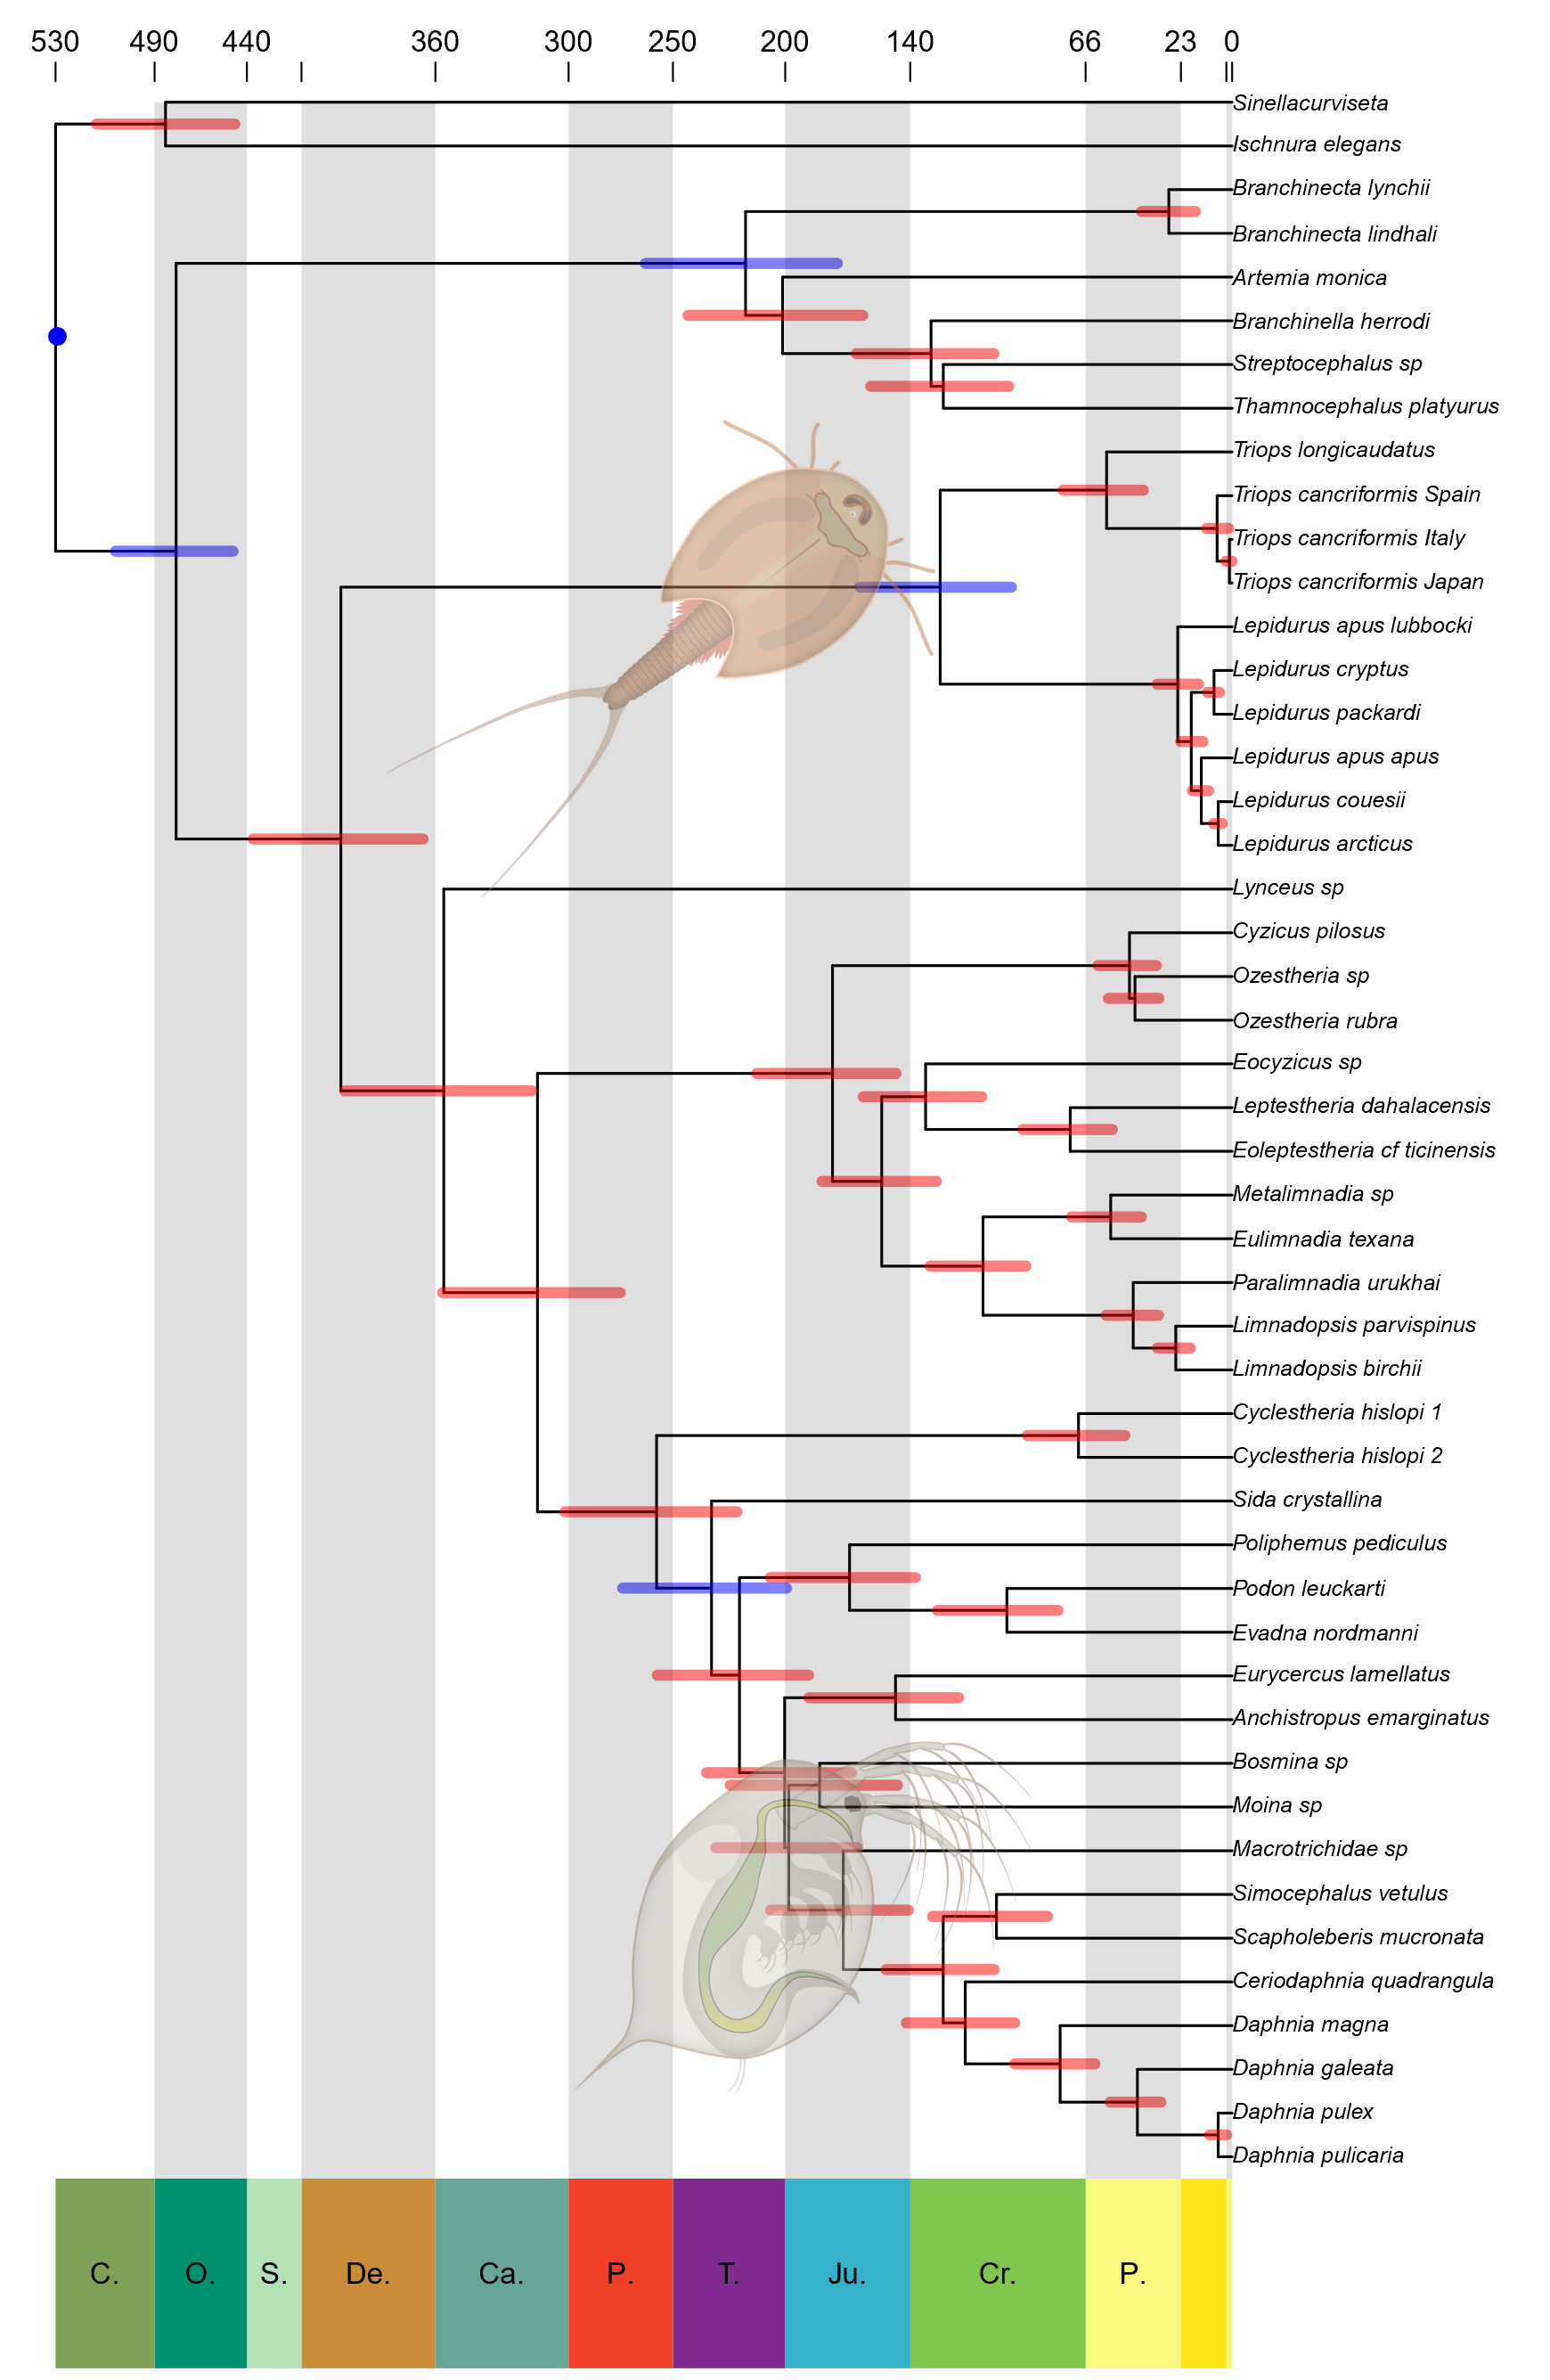
\includegraphics[width=0.65\textwidth]{Figures/lsd2tree_2.0.png}
    \caption[Tree dated with lsd2]{Tree dated with lsd2: blue bars are the prior calibrations. The two silhouettes represent the most studied groups of branchiopods, on top Notostraca and at the bottom Cladocera.
}
    \label{fig:lsd2tree}
\end{figure}

\begin{figure}[h!]
    \centering
    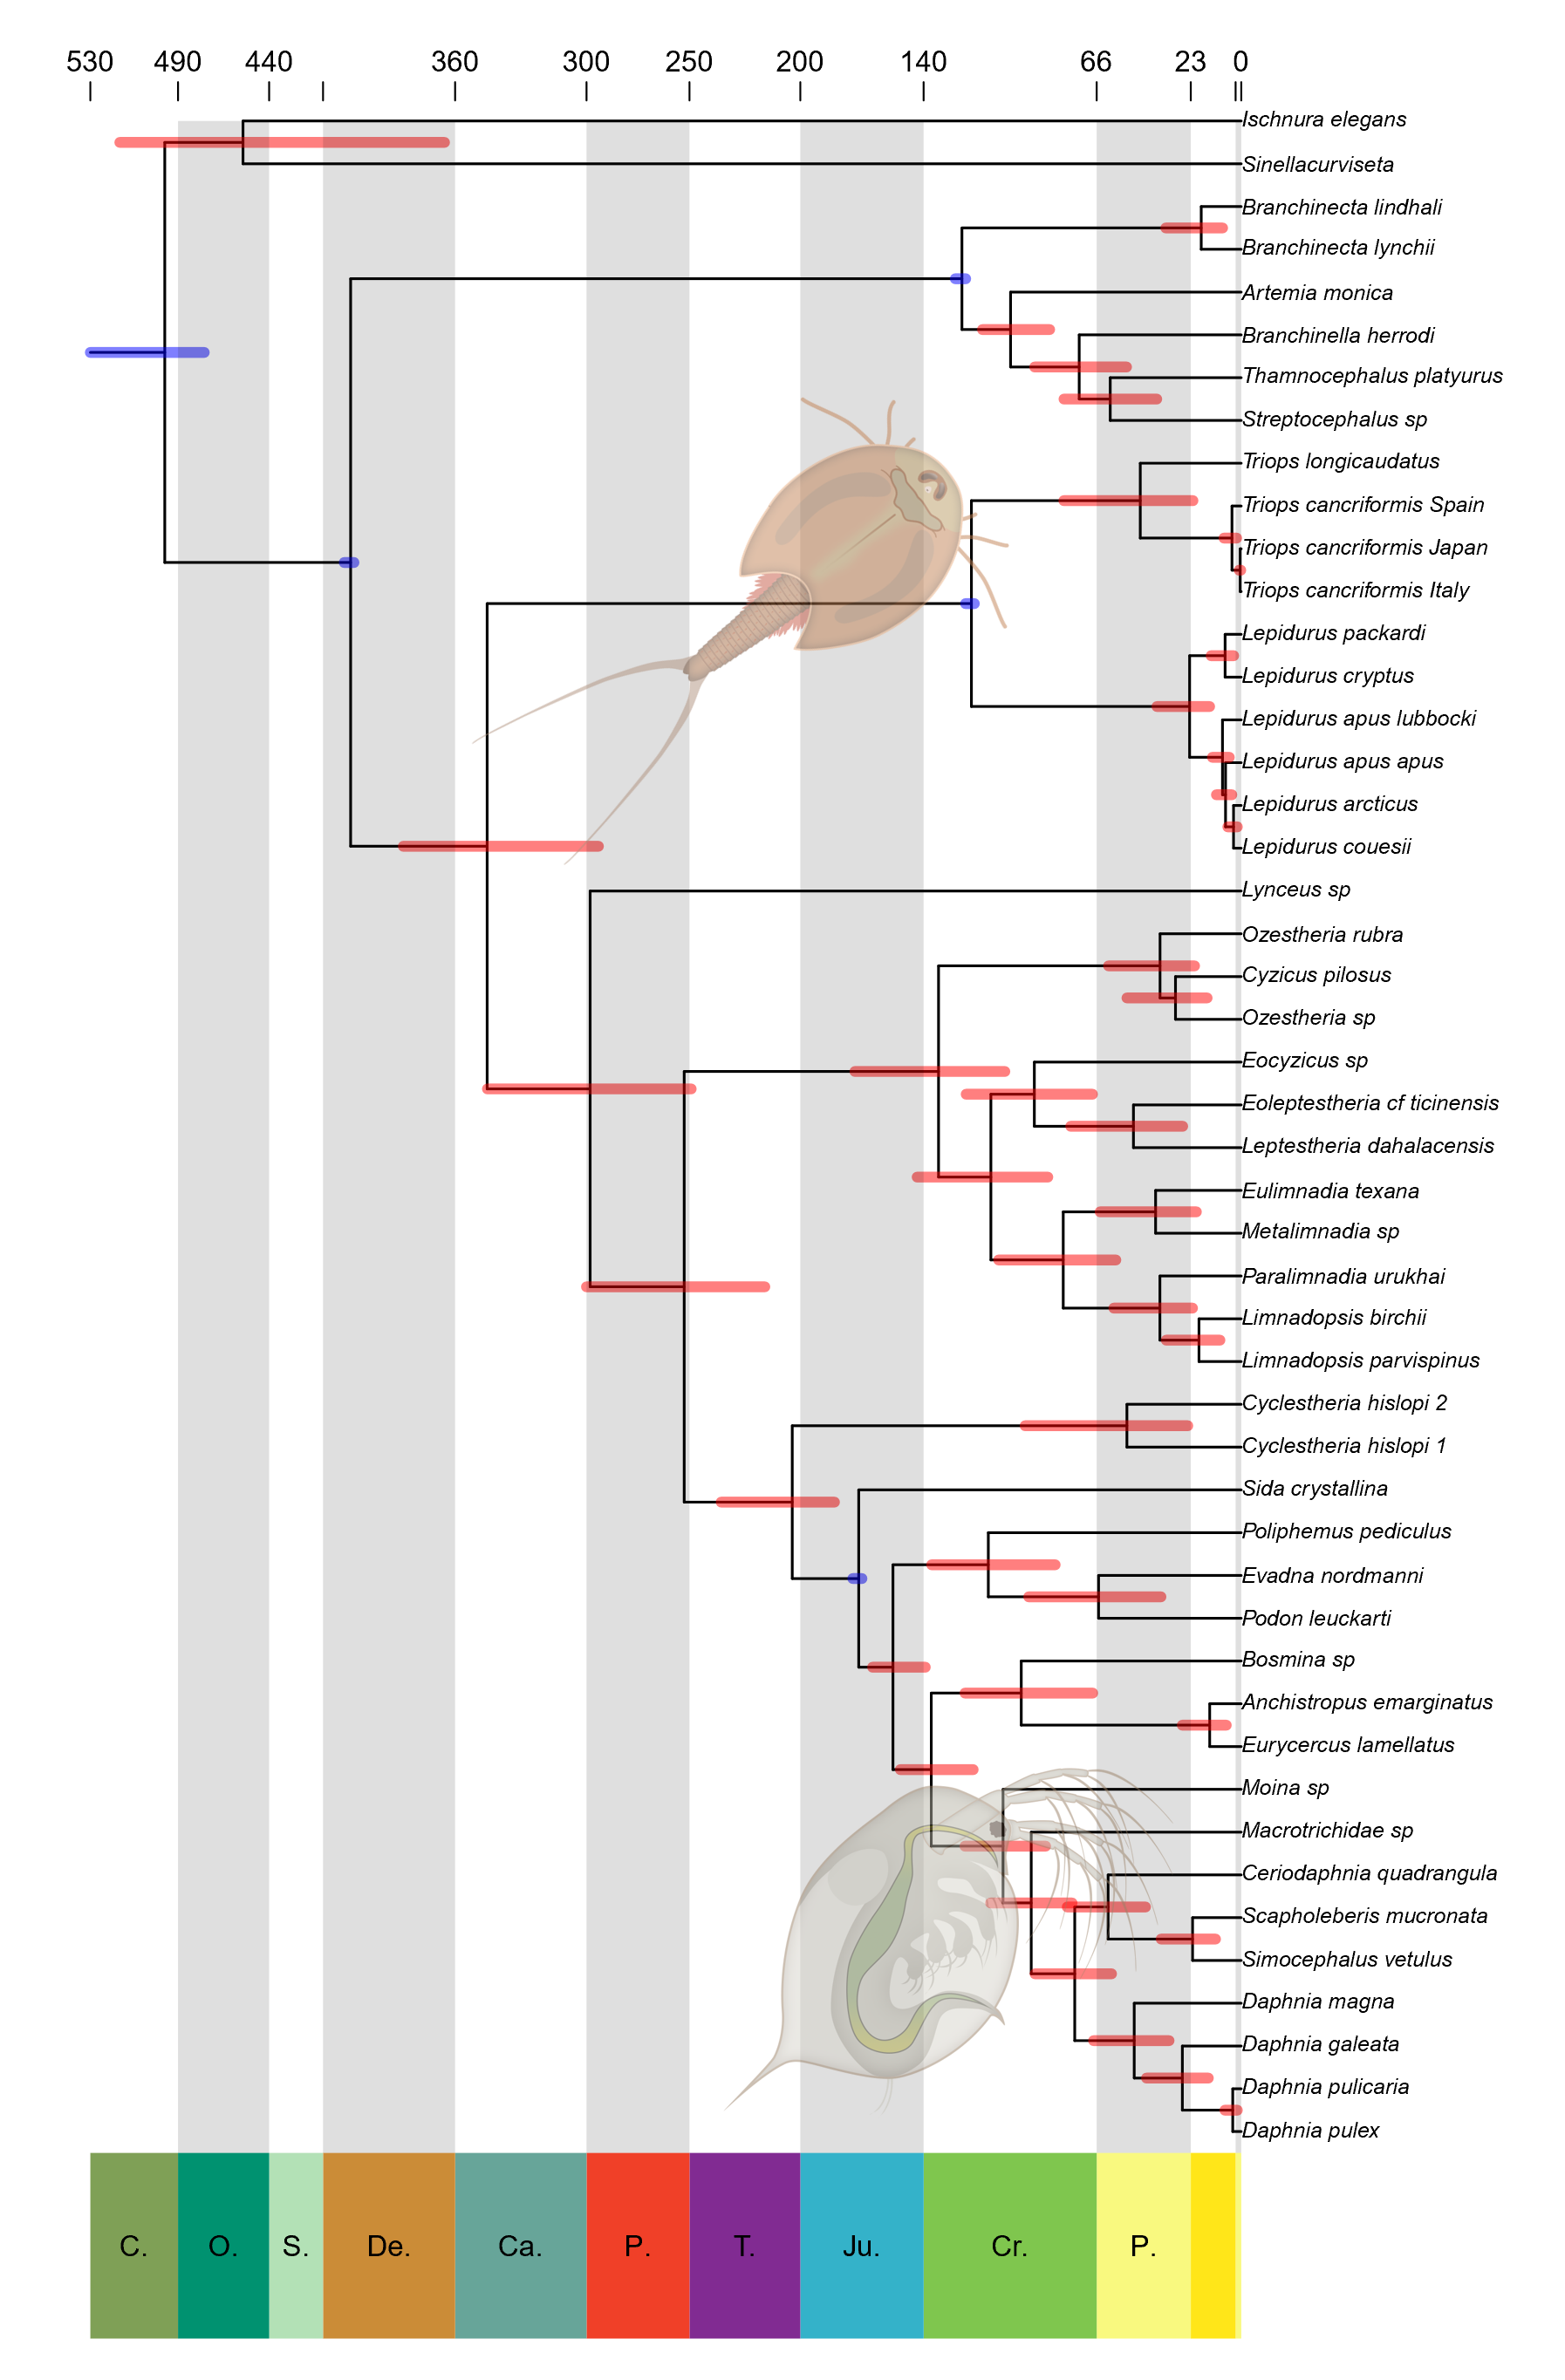
\includegraphics[width=0.7\textwidth]{Figures/mcmctree_gbm_2.0.png}
    \caption[Tree dated with MCMCtree with GBM Clock Model]{Tree dated with MCMCtree with correlated rates (GBM) Clock Model: blue bars are the prior calibrations. The two silhouettes represent the most studied groups of branchiopods, on top Notostraca and at the bottom Cladocera.
}
    \label{fig:mcmctree_gbm}
\end{figure}


\begin{figure}[h!]
    \centering
    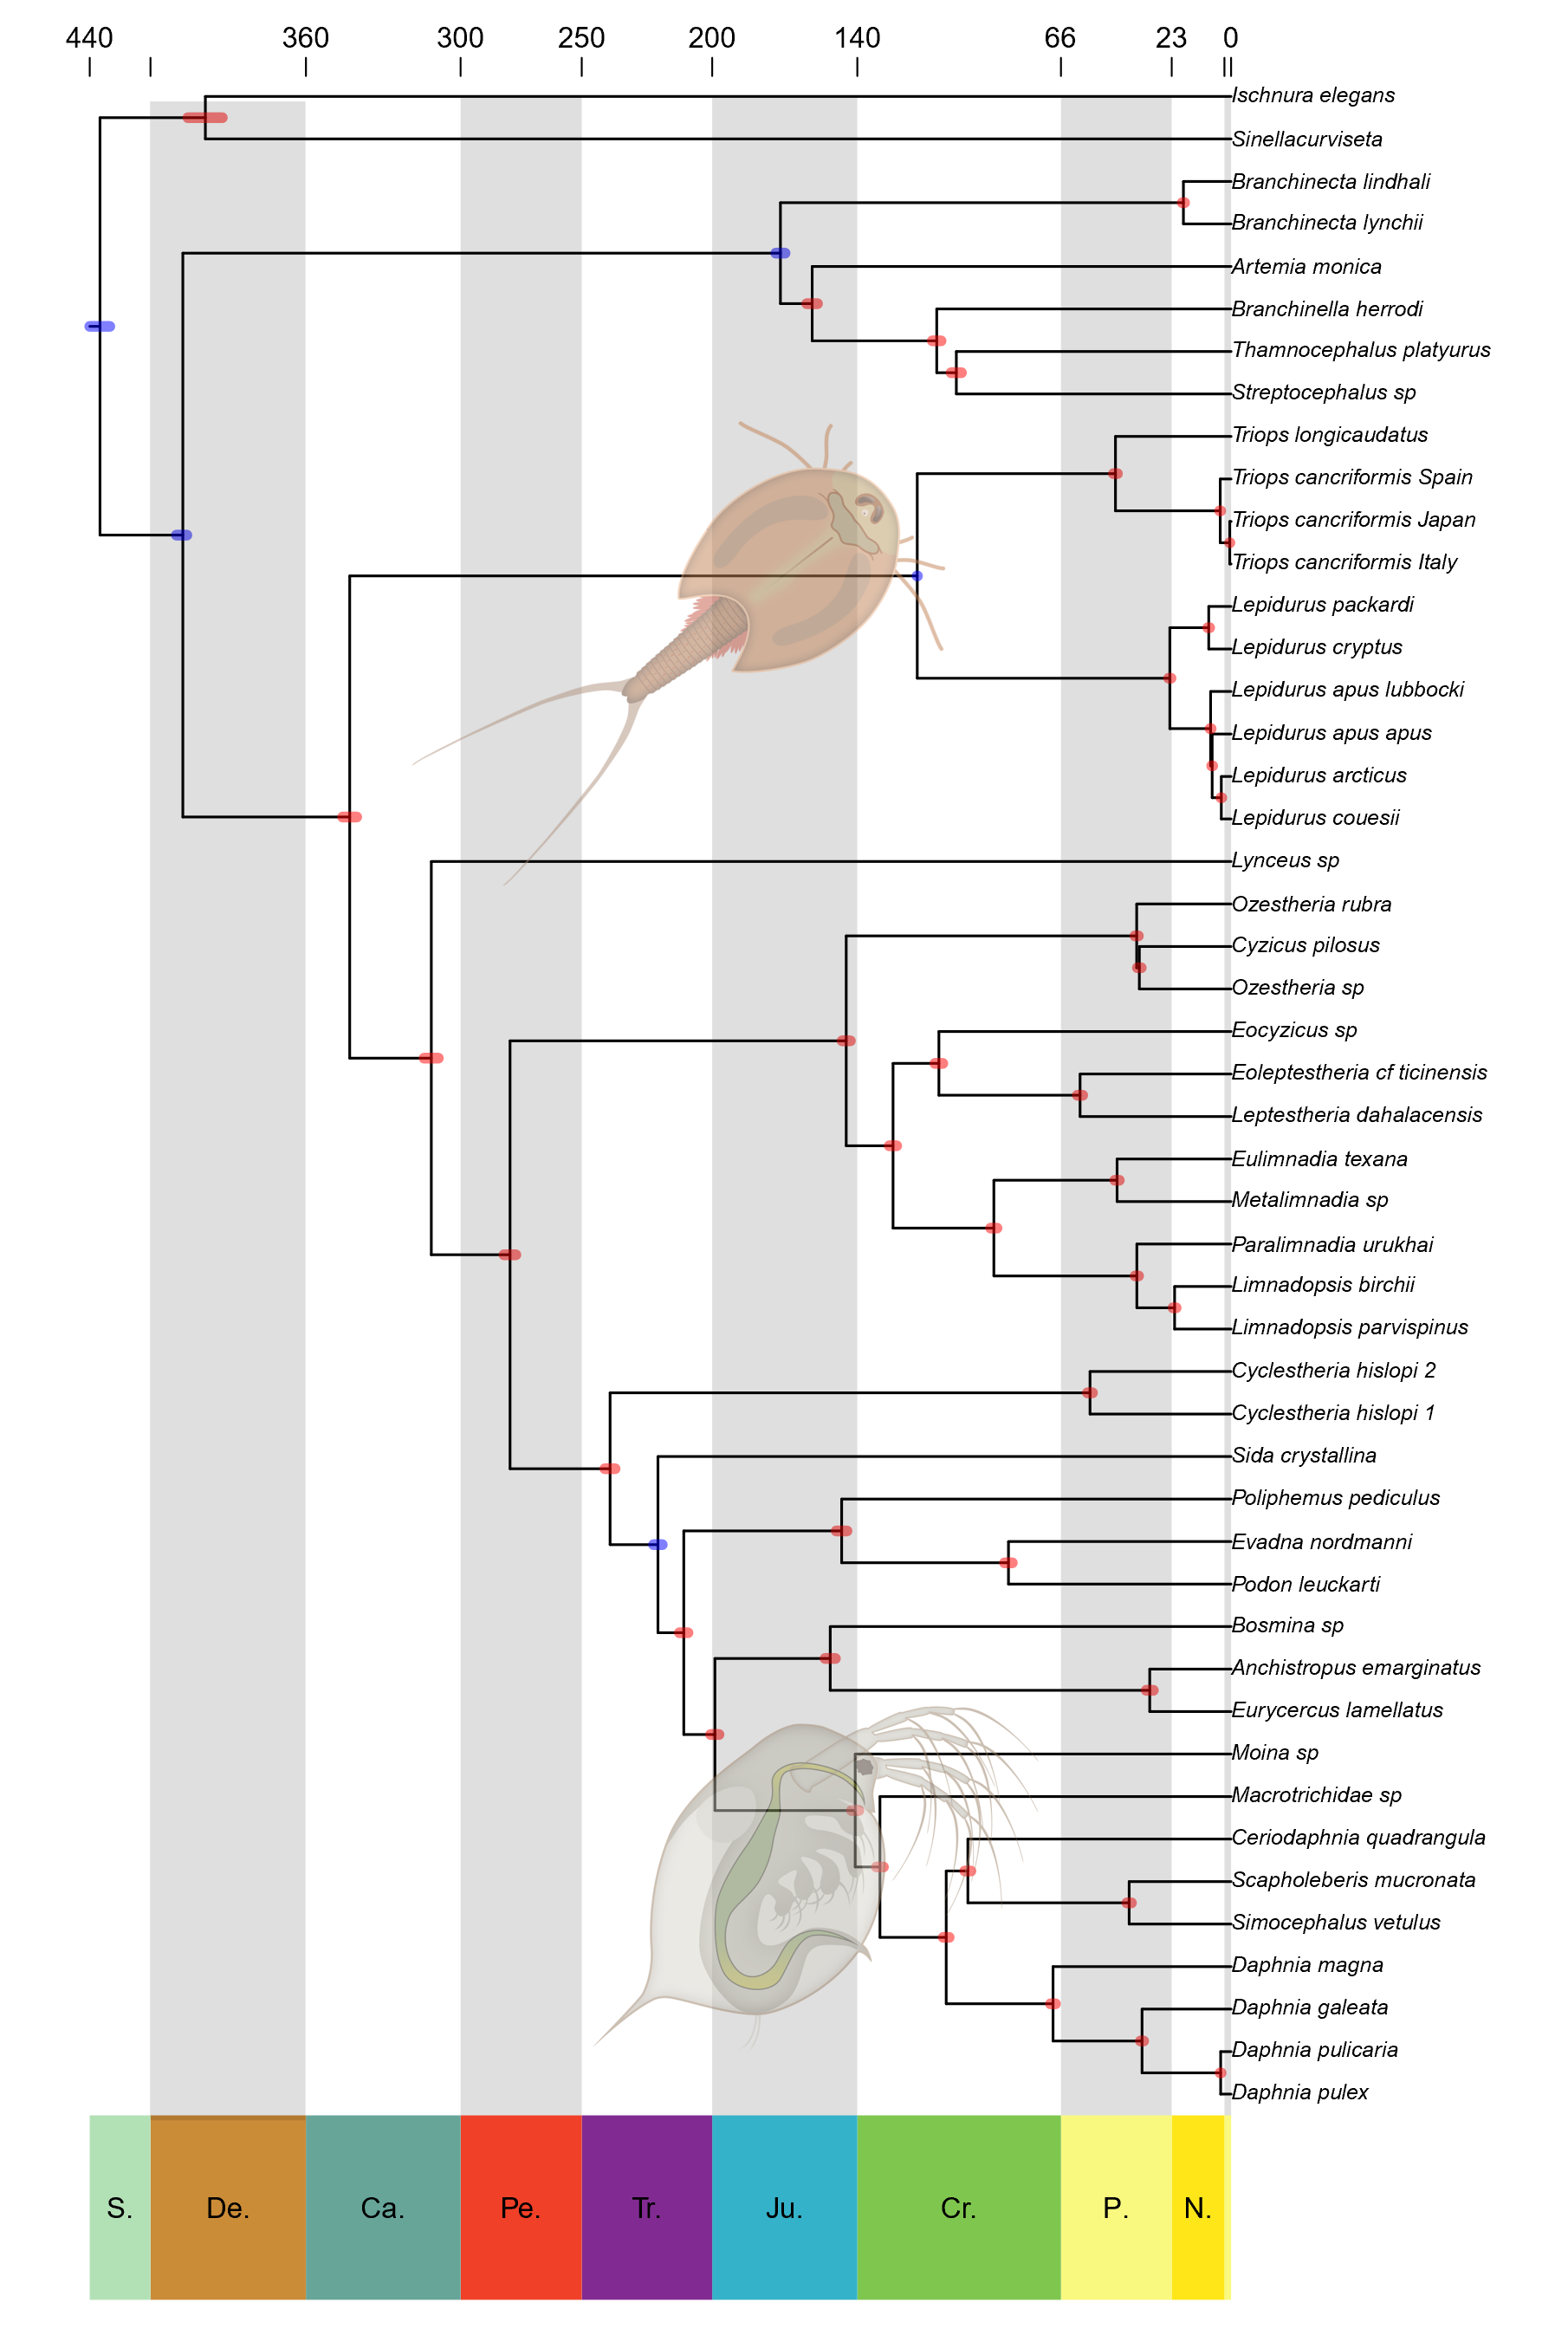
\includegraphics[width=0.7\textwidth]{Figures/mcmctree_strict_2.0.png}
    \caption[Tree dated with MCMCtree with strict Clock Model]{Tree dated with MCMCtree with global (strict) Clock Model: blue bars are the prior calibrations. The two silhouettes represent the most studied groups of branchiopods, on top Notostraca and at the bottom Cladocera.
}
    \label{fig:mcmctree_strict}
\end{figure}


\begin{figure}[h!]
    \centering
    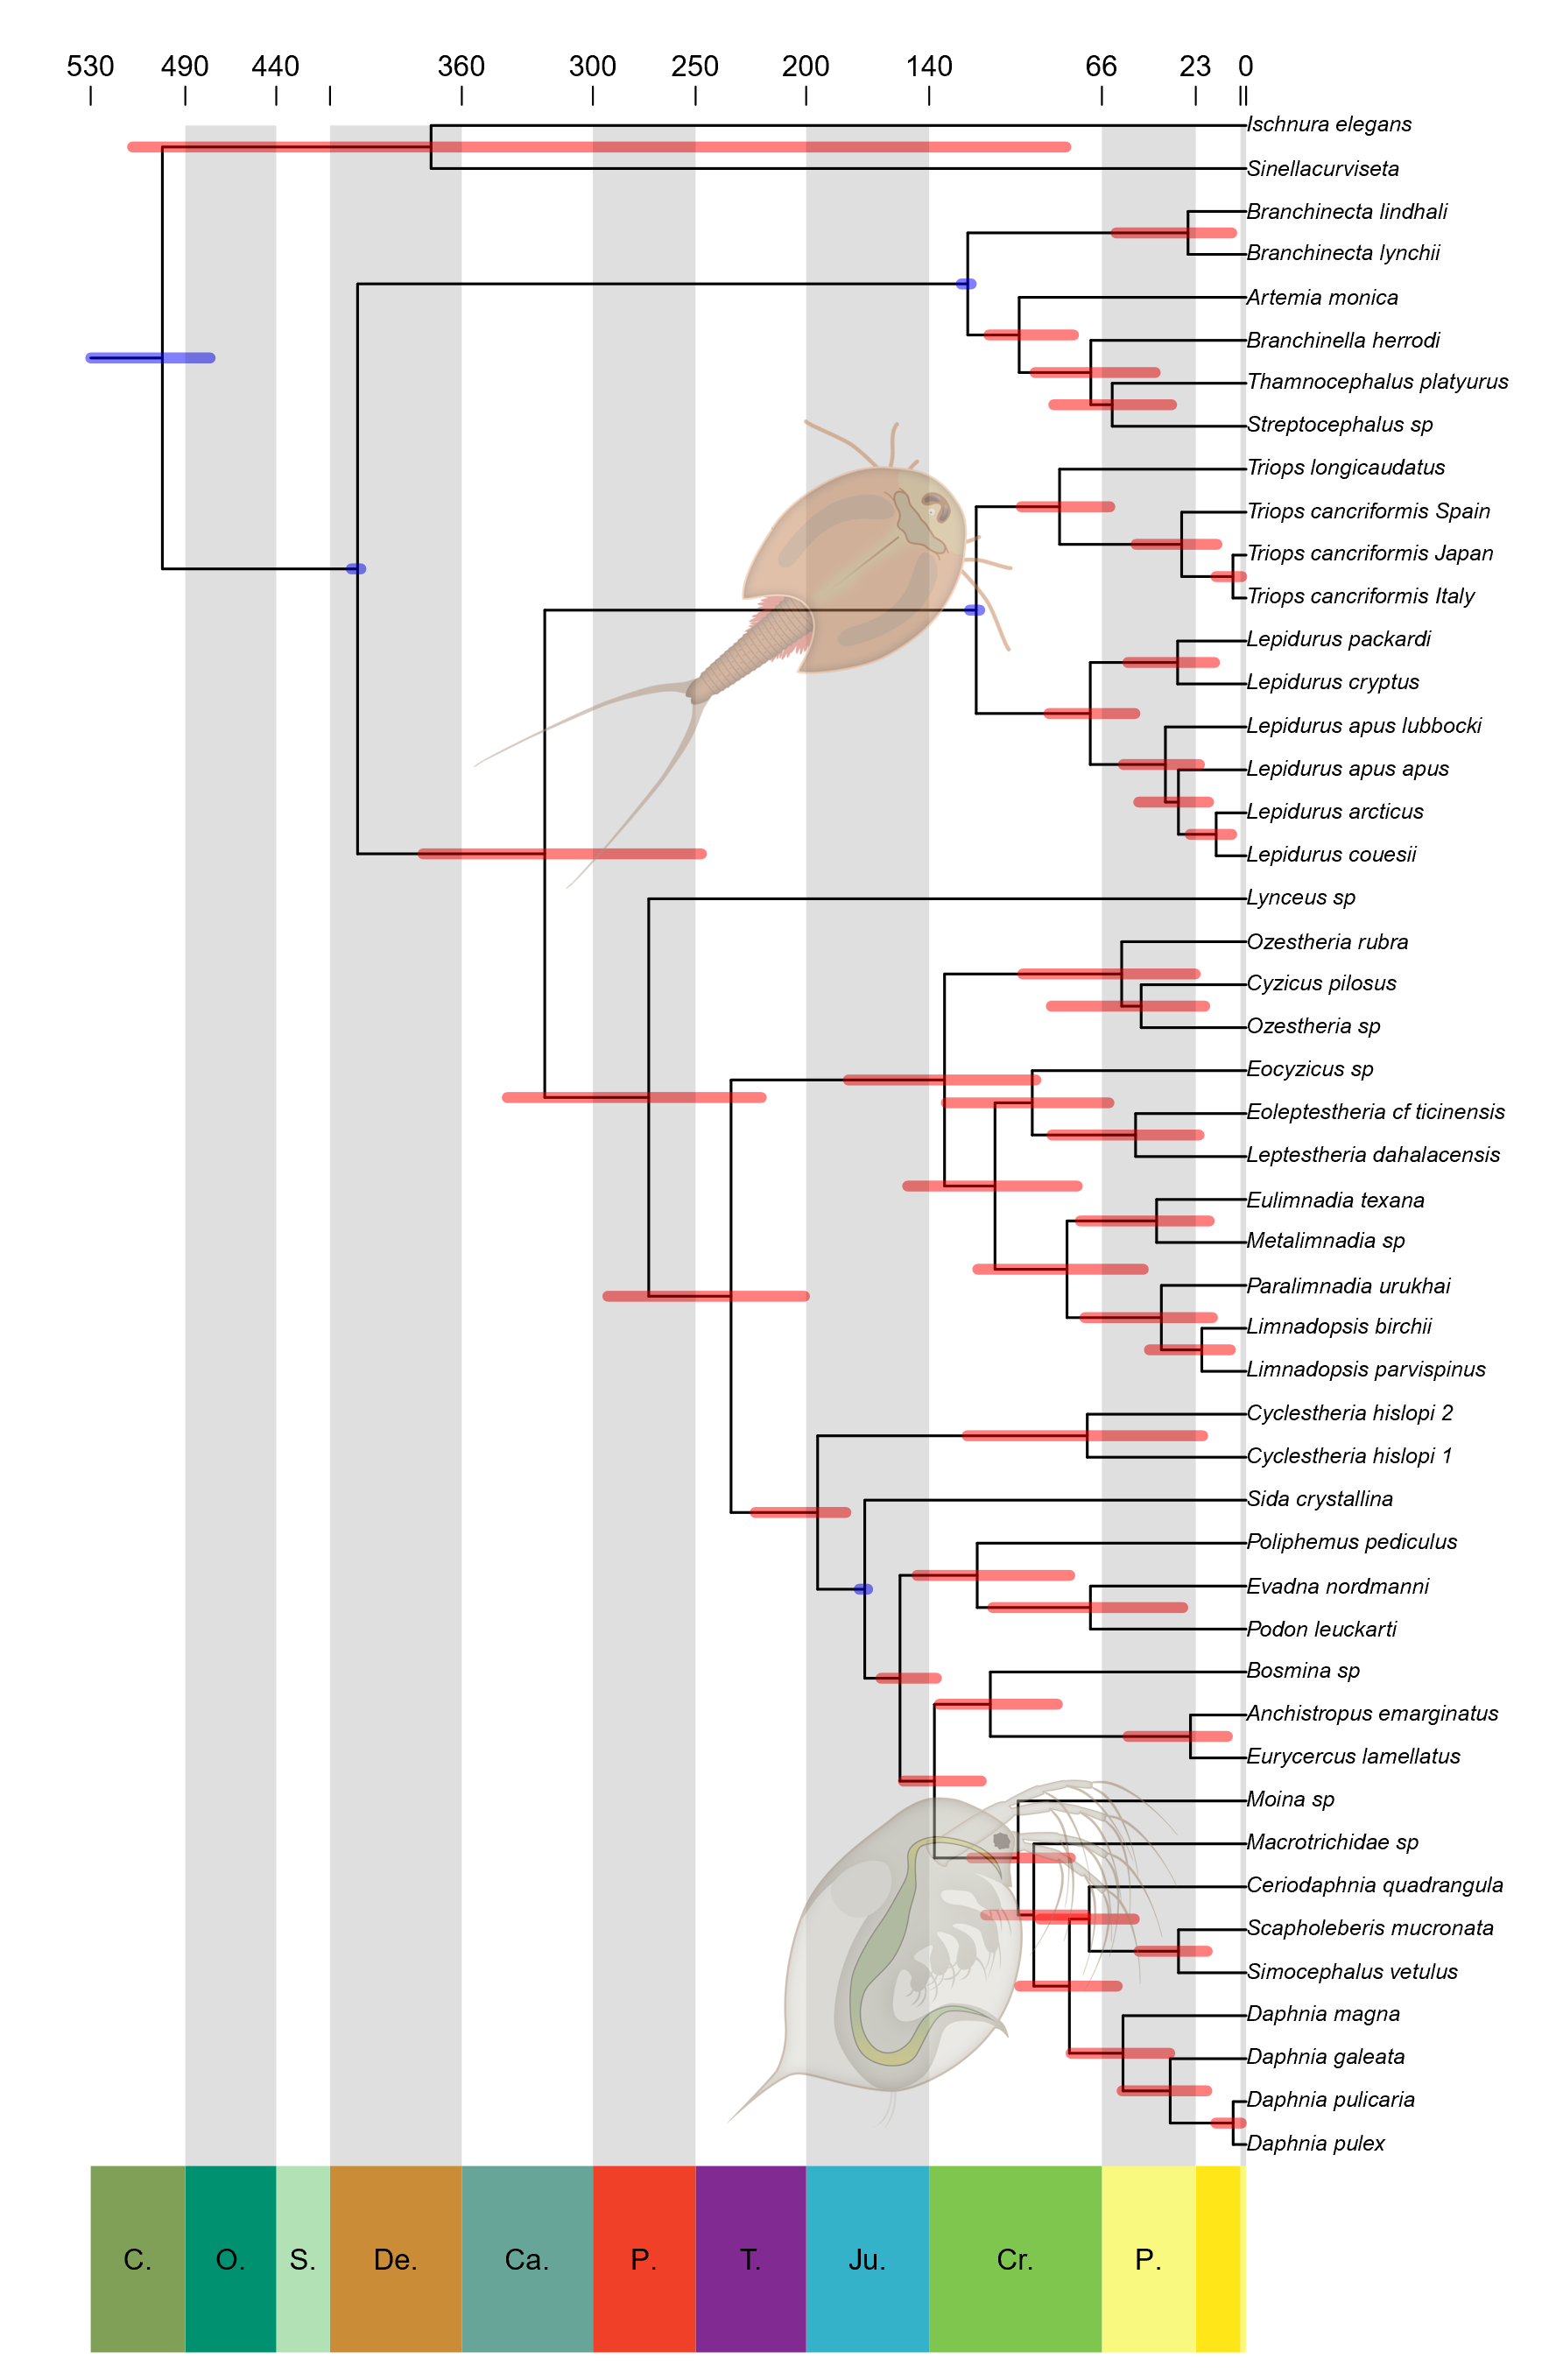
\includegraphics[width=0.7\textwidth]{Figures/mcmctree_iln_2.0.png}
    \caption[Tree dated with MCMCtree with independent rates (ILN) Clock Model]{Tree dated with MCMCtree with ILN Clock Model: blue bars are the prior calibrations. The two silhouettes represent the most studied groups of branchiopods, on top Notostraca and at the bottom Cladocera.
}
    \label{fig:mcmctree_iln}
\end{figure}

\begin{figure}[ht]
    \centering
    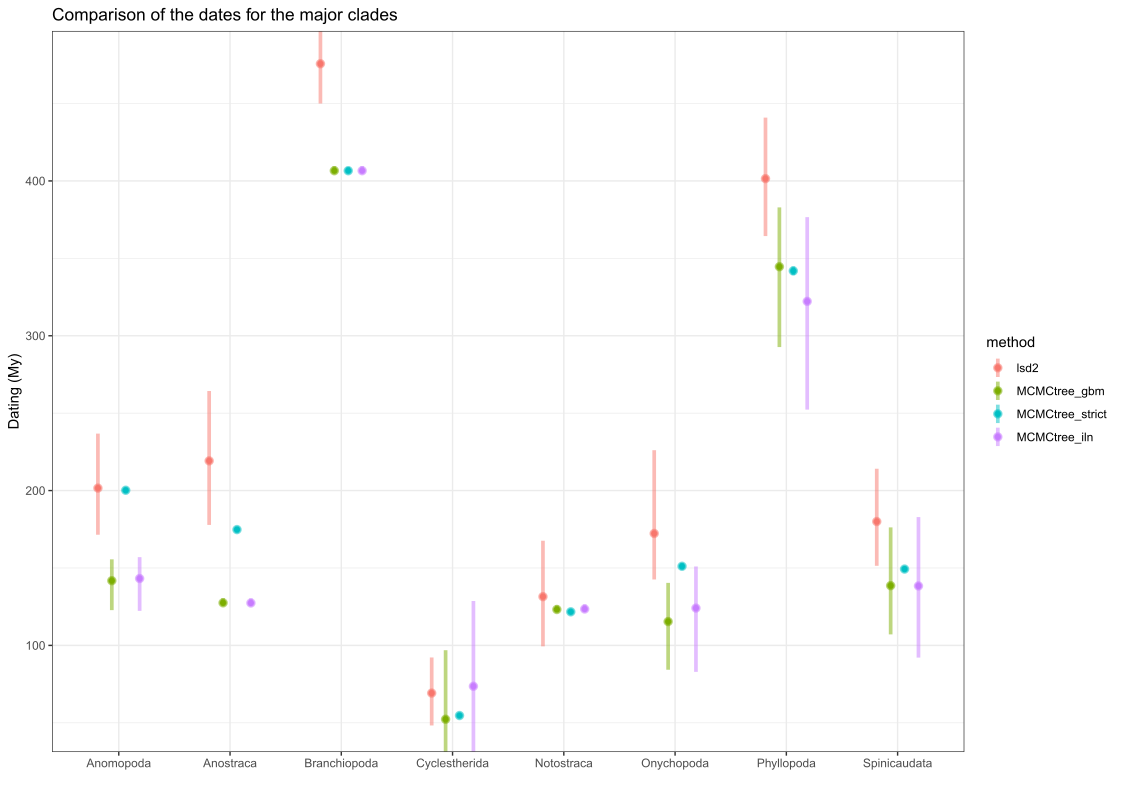
\includegraphics[width=1\textwidth]{Figures/dates_comparison.png}
    \caption[Comparison of the dates for the major clades)]{Comparison of the dating of the major clades of Branchiopoda with 4 different methods (i.e., lsd2 and MCMCtree with GBM, strict, and ILN clock models) with confidence intervals.
}
    \label{fig:dating_comparison}
\end{figure}